\documentclass[a4paper,11pt]{article}

%=========================
% Les styles
%=========================
\usepackage{style-esi/french}	% Francise LaTeX
\usepackage{style-esi/td}
\usepackage{style-esi/licence}	% Affiche une licence dans le document
\usepackage{style-esi/exercice}
\usepackage{style-esi/exemple}
\usepackage{style-esi/listing}
\usepackage{style-esi/tutoriel}
\usepackage{style-esi/terminal}
\usepackage{booktabs}
\usepackage{pifont} 
\usepackage{longtable}
\usepackage{pdfpages}
\usepackage{minitoc}
\setcounter{secttocdepth}{3}
\usepackage{tikzpeople}
\let\oldhref\href
\renewcommand{\href}[2]{\oldhref{#1}{#2}\footnote{\url{#1}}} 

\definecolor{verylightgray}{rgb}{0.98,0.98,0.98}

\date{2018 -- 2019}
\siglecours{DEV1}
\libellecours{Laboratoires d'environnement}
\libelledocument{TD 08 -- Secure Shell} \sigleprof{}
\sigleprof{}



\begin{document}

\entete
\titre
\ccbysa{esi-dev1-list@he2b.be}
\lastedit

\dosecttoc
\setcounter{tocdepth}{1} 
\mtcsettitle{secttoc}{}


\begin{tcolorbox}
	[blanker, before skip=10mm,after skip=10mm, 
		borderline west={1mm}{-4mm}{lightgray},
		title=Objectifs, coltitle=black, fonttitle=\sffamily\bfseries\large]

		À la fin de ce module, vous pourrez différencier les étapes et systèmes
		intervenants dans une connexion \textit{ssh}, utiliser et configurer la
		commande \textit{ssh} et différentes options dans différents contextes et
		décrire les algorithmes sous-jacents. 

\end{tcolorbox}

\vspace{-12mm}
\renewcommand{\contentsname}{}
\tableofcontents
\vspace{5mm}

\emph{Secure SHell} (\emph{ssh}) permet d'obtenir un \textbf{\emph{shell}}
\textbf{sécurisé} à distance~:

\begin{itemize}

	\item un \textbf{\emph{shell}} --- comme \emph{bash} --- est un interprèteur
		de commandes. C'est lui l'interface entre l'utilisateur et le système
		d'exploitation. Il est en mode texte.

	\item il est \textbf{sécurisé} parce que les messages échangés sont
		chiffrés. Il offre les fonctionnalités suivantes~:

		\begin{enumerate}
			\item l'authentification du serveur;
			\item la confidentialité des données échangées (ou session chiffrée);
			\item l'intégrité des données échangées;
			\item l'authentification du client.
		\end{enumerate}

\end{itemize}


\emph{ssh} fonctionne en «~client-serveur~»~:

\begin{itemize}

	\item un programme sur l'une des machines est le \textbf{client};

		Ce \emph{client} se connecte au serveur. Il ouvre un canal de
		communication vers une certaine adresse et envoie un message de demande
		de connexion. Il envoie également des identifiants de connexion.  

	\item un programme sur l'autre machine est le \textbf{serveur};

		Ce \emph{serveur} écoute continuellement les demandes de connexion.  Dès
		qu'un message lui parvient, le \emph{serveur} échange des données avec
		le \emph{client}.

		Ce programme exécuté en tâche de fond, c'est un \emph{dæmon}, écoute
		(généralement) les demandes de connexion. Dès que le client
		s'authentifie correctement, le programme fournit l'environnement --- un
		\emph{shell} --- prévu.

\end{itemize}

Lorsque la communication est chiffrée, un utilisateur malveillant ne pourra pas
écouter cette communication. Plus précisément, il pourra peut-être l'écouter
mais ne la comprendra pas sans les codes d'accès appropriés. 




\section{Vocabulaire}
\label{vocabulaire}

\secttoc

\subsection{Chiffrement symétrique}
\label{chiffrement-symétrique}

Le \textbf{chiffrement symétrique}, appelé aussi chiffrement par échange
d'une clé ou par clé partagée ou encore par clé secrète, est un système
qui consiste au chiffrement des messages échangés, avec une clé de
chiffrement commune et partagée «~à l'avance~» par les intervenants.

\begin{center}
\begin{tikzpicture}[every node/.style={minimum width=1.5cm}]
    \draw (0,0) node[alice] (alice) 
    {
        \begin{tabular}{c}
			\textbf{Alice} \\ 
			Chiffre avec la clé \\ 
			\faKey\,\textit{secret partagé}
        \end{tabular}
    };
    \draw (8,0) node[bob, shirt=purple, mirrored] (bob) 
    {
        \begin{tabular}{c}
        	\textbf{Bob} \\ 
        	Déchiffre avec la clé \\ 
        	\faKey\,\textit{secret partagé}
        \end{tabular}
    };
	\draw (4.7,-3.5) node[bob, female, shirt=black, mirrored ] (eve) 
	{
		\begin{tabular}{c}
			\textbf{Ève} \\
			Ne peut comprendre le message. \\
			Elle ne peut pas le déchiffrer sans la clé.
		\end{tabular}
	};
	\draw[->, thick] (alice) -- (bob) node[above, midway] {WW91IGdldCBpdCAhCg==};
	\draw[->, dotted] (eve) -- (4,-0.2) node[right=-5mm, midway] {\textbf{?}};
\end{tikzpicture}
\end{center}
\vspace{2cm}

Voici quelques noms d'algorithmes de chiffrements symétriques% 
\footnote{Cette liste est accessible par la commande \texttt{ssh\ -Q\ cipher}
depuis OpenSSH v7}~: 3des-cbc blowfish-cbc cast128-cbc arcfour arcfour128
arcfour256 aes128-cbc aes192-cbc aes256-cbc rijndael-cbc@lysator.liu.se
aes128-ctr aes192-ctr aes256-ctr aes128-gcm@openssh.com aes256-gcm\-@openssh.com
chacha20-poly1305@openssh.com

\bigskip
\begin{Exercice}*{Chiffrement, déchiffrement}    
    La commande `openssl` permet d'encoder (chiffrer) et déchiffrer un texte.
    Voyons ça:
	
	\begin{itemize}
    	\item créez et éditez un fichier nommé `mysecrets` contenant quelques 
    		phrases;
    
    	\item chiffrez ce fichier (vous devrez entrer un mot de passe);

			\begin{term}
			openssl enc -aes-256-cbc -out mysecrets.ciphered
			   -in mysecrets
			\end{term}

		\item observez le contenu du fichier chiffré;

			\pagebreak
		\item déchiffrez-le et affichez le contenu déchiffré sur la sortie 
			standard;
			
			\begin{term}
			openssl enc -aes-256-cbc -in mysecrets.ciphered -d
	        \end{term}
	
	\end{itemize}

\end{Exercice}




\subsection{Chiffrement asymétrique}
\label{chiffrement-asymétrique}

Le \textbf{chiffrement asymétrique} appelé aussi chiffrement à clé publique est
un système qui consiste au chiffrement des messages échangés, à l'aide de
plusieurs clés. 

Supposons qu'Alice veuille envoyer un message à Bob de manière confidentielle et
qu'ils ne détiennent pas de clé secrète partagée. Ils ne peuvent pas faire
transiter la (future) clé secrète sur le canal non sûr par peur que cette clé ne
soit interceptée. Le chiffrement asymétrique peut venir à leur secours. 

\begin{center}
\begin{tikzpicture}[every node/.style={minimum width=1.5cm}]
    \draw (0,0) node[alice] (alice) 
    {
        \begin{tabular}{c}
			\textbf{Alice} \\
			({\color{red}\faKey}\,$Alice_{Pr}$, 
			{\color{green!70!black}\faKey}\,$Alice_{Pu}$) \\
			Chiffre avec la {\color{green!70!black}\faKey}\, $Bob_{Pu}$ 
		\end{tabular}
    };
    \draw (8,0) node[bob, shirt=purple, mirrored] (bob) 
    {
        \begin{tabular}{c}
			\textbf{Bob} \\ 
			({\color{red}\faKey}\,$Bob_{Pr}$, 
			{\color{green!70!black}\faKey}\,$Bob_{Pu}$) \\
			Déchiffre avec sa {\color{red}\faKey}\,$Bob_{Pr}$
        \end{tabular}
    };
	\draw (4.7,-4) node[bob, female, shirt=black, mirrored ] (eve) 
	{
		\begin{tabular}{c}
			\textbf{Ève}
		\end{tabular}
	};
	\draw[->, thick] (alice) -- (bob) node[above, midway] 
		{HRIx6HSVanbEaV+JVi3(cut)};
	\draw[->, dotted] (eve) -- (4,-0.2) node[right=-5mm, midway] {\textbf{?}};
\end{tikzpicture}
\end{center}

\vspace{2cm}


Alice et Bob possèdent chacun deux clés — une clé publique
({\color{green!70!black}\faKey}\,$Pu$) et une clé privée
({\color{red}\faKey}\,$Pr$) — telles que~:

\begin{itemize}
	\item il est rapide de chiffrer un message avec la clé publique ;
	
	\item il est rapide de déchiffrer le message avec la clé privée~;

	\item il est impossible en un temps raisonnable de déchiffrer le
		message avec la clé publique ou de déduire la clé privée à partir de la 
		clé publique.

\end{itemize}

Dans ces conditions, il suffit de publier sa clé publique et de conserver
précieusement sa clé privée. Toute personne voulant m'envoyer un message le
chiffrera avec ma clé publique… et je le déchiffrerai avec ma clé privée. 


Voici quelques noms d'algorithmes de chiffrements asymétriques
~: RSA, DSA, ECDSA. 
	
\begin{coltbox}{Remarque}	
	Il est possible de générer une clé RSA|DSA avec \texttt{ssh-keygen} et
	\texttt{openssl}. Les deux programmes génèreront une clé privée de format et
	de taille voulue.

	\begin{itemize}
		\item \texttt{ssh-keygen} génèrera directement la clé publique au
			format \textit{OpenSSH}
		\item \texttt{openssl} ne génèrera pas de clé publique
			automatiquement… mais il est possible de le lui demander. Dans ce
			cas, cette clé sera au format PEM.
	\end{itemize}
\end{coltbox}
\vspace{1cm}

\begin{Exercice}*{Chiffrement, déchiffrement asymétrique}
	La commande \texttt{openssl} permet toujours de chiffrer et déchiffrer un 
	message… cette fois de manière asymétrique. 

	\textit{Vous pouvez faire cet exercice avec votre voisin ou voisine.}

	
	Faites donc~:

	\begin{itemize}
		
		\item générez une paire de clé \textit{ssh} si vous ne l'avez pas déjà
			fait. Pour RSA 4096 bits la commande suivante créera deux fichiers~;
			\texttt{id\_rsa} et \texttt{id\_rsa.pub}.

			\begin{term}
				ssh-keygen -t rsa -b 4096
			\end{term}

			Regardez quelles permissions ces fichiers ont. 

		\item le format OpenSSH de la clé publique ne conviendra pas pour la
			suite, créons un fichier contenant cette même clé au format PEM;

			\begin{term}
				openssl rsa -in id\_rsa -pubout -out id\_rsa.pub.pem
			\end{term}

		\item vous pouvez «~diffuser~» votre clé publique  (en la mettant dans 
			un répertoire accessible par votre voisin·e, il ou elle pourra 
			l'utiliser par exemple); 

		\item chiffrez un message avec une clé publique (celle de votre voisin·e
			par exemple) et partagez le message chiffré;

			\begin{term}
				echo "Message super secret" 
				    | openssl pkeyutl -encrypt -pubin 
				        -inkey <la clé publique du voisin> 
				        -out encrypted-message.bin
			\end{term}

		\item cherchez dans la page de manuel de \texttt{openssl} comment 
			déchiffrer le message avec votre clé privée… et déchiffrez le 
			message reçu de votre voisin·e. 

	\end{itemize}

\end{Exercice}





\subsection{Signature des messages}
\label{signature}

Pour vérifier l'intégrité d'un message lors de sa transmission, le message est
signé. Cette signature atteste que le message (chiffré) transmis n'a pas été
altéré pendant le transport. 

Cette signature — généralement plus courte que le message lui-même — accompagne
le message. Le récepteur du message signe le message reçu et compare la
signature reçue avec la signature qu'il vient de calculer. 

Cette signature MAC (\textit{message authentication code}) peut s'accompagner
d'une clé secrète, on parle alors de HMAC (\textit{keyed-hash message
authentication code}). Dans le cas de \textit{ssh}, c'est bien HMAC qui est
utilisé avec la clé de session (cfr section \ref{comment-se-passe-la-connexion}). 

Voici quelques algorithmes \texttt{HMAC}
\footnote{Accessible par la commande \texttt{ssh -Q mac}}~:
hmac-sha1 hmac-sha1-96 hmac-sha2-256 hmac-sha2-512 hmac-md5 hmac-md5-96
hmac-ripemd160 hmac-ripemd160@openssh.com umac-64\-@openssh.com
umac-128@openssh.com hmac-sha1-etm@openssh.com hmac-sha1-96-etm\-@openssh.com
hmac-sha2-256-etm@openssh.com hmac-sha2-512-etm@openssh.com
h\-mac-md5-etm@openssh.com hmac-md5-96-etm@openssh.com
hmac-ripemd160-etm\-@o\-penssh.com umac-64-etm@openssh.com umac-128-etm@openssh.com

\bigskip
\begin{Exercice}*{Altération d'un message}
	Vérifions l'intégrité d'un message avec SHA-512. 

	\begin{itemize}
	
		\item éditez un nouveau fichier en y écrivant quelques lignes de texte;
		\item calculez le \textit{hash} du message; 

			\begin{term}
				sha512sum <fichier>
			\end{term}

		\item modifiez un caractère de votre fichier, recalculez le
			\textit{hash} et constatez les différences (ou plus exactement,
			cherchez une similitude).
	\end{itemize}

	Ceci montre que si le message est altéré — même très peu — son \textit{hash}
	est complètement différent. En regardant le \textit{hash}, il est donc très
	facile et rapide de vérifier l'intégrité du message. 

\end{Exercice}

\bigskip
\bigskip
\begin{coltbox}{Remarque}	

	Cette technique est utilisée lors du téléchargement de certains fichiers par
	exemple. Ces fichiers sont accompagnés d'un \textit{hash} qu'il est facile
	de vérifier. 

	Dans certains cas, le \textit{hash} est disponible sur le site officiel et
	le fichier est répliqué à différents endroits. Vérifier le \textit{hash}
	permet d'être sûr que le fichier n'a pas été altéré lorsqu'il a été partagé
	sur un autre site.  

\end{coltbox}

\clearpage \begin{Exercice}*{Vérification d'une archive} À l'adresse
	\url{https://cdimage.debian.org/debian-cd/current/amd64/iso-cd}, vous
	trouverez en téléchargement des \textit{iso}\footnote{Une \textit{iso} est
un fichier contenant toute une arborescance de fichier. Initialement prévu pour
être gravé sur un cdrom ou un dvd, il peut aujourd'hui être placé sur n'importe
quel support amovible ou remplacer un lecteur DVD dans une machine virtuelle.}
debian à télécharger. 
	
	Ces fichiers sont accompanés de fichiers de somme de contrôle
	(\textit{hash}).  Ces \textit{hashs} servent à vérifier l'intégrité de
	l'\textit{iso} téléchargé.

	\begin{enumerate}

		\item Téléchargez la plus petite iso correspondant au \textit{pattern}
			(schéma) \\\texttt{debian*-netinst.iso};

		\item calculez le \textit{hash} du fichier à l'aide d'une des commandes
			\texttt{sha512sum}, \texttt{sha256sum} voire \texttt{md5sum};

		\item comparez la valeur obtenue avec la valeur se trouvant dans le
			fichier correspondant au \textit{hash} que vous avez choisi;

			\medskip
			Si les valeurs correspondent, c'est que le fichier téléchargé est
			bien le fichier qui a été déposé par les responsables debian… sinon,
			ne l'utilisez pas. 
			\medskip

		\item effacez le fichier que vous venez de télécharger \footnote{Cette
			étape est importante pour éviter que ce fichier de près de 300Mib
			reste en beaucoup d'exemplaire sur linux1. Merci de la part des
			administrateurs de cette machine.}

	\end{enumerate}

	Pour être complet, il faudrait également vérifier que ces fichiers de somme
	de contrôle sont eux-même corrects… mais ça sort du cadre de ce premier td.
	Le lecteur intéressé suivra \href{https://www.debian.org/CD/verify}{le lien}
	renseigné sur le site de debian. 
	
\end{Exercice}



\section{Comment se passe la connexion ?}
\label{comment-se-passe-la-connexion}

Extrait d'une page de manuel de \texttt{sshd}~:

\begin{quote}

	\it\small
	The OpenSSH SSH daemon supports SSH protocol 2 only.  Each host has a host-
	specific key, used to identify the host.  Whenever a client connects, the
	daemon responds with its public host key.  The client compares the host
	key against its own database to verify that it has not changed.  Forward
	security is provided through a Diffie-Hellman key agreement.  This key
	agreement results in a shared session key.  The rest of the session is
	encrypted using a symmetric cipher, currently 128-bit AES, Blowfish, 3DES,
	CAST128, Arcfour, 192-bit AES, or 256-bit AES.  The client selects the
	encryption algorithm to use from those offered by the server.  Additionally,
	session integrity is provided through a cryptographic message
	authentication code (hmac-md5, hmac- sha1, umac-64, umac-128,
	hmac-ripemd160, hmac-sha2-256 or hmac-sha2-512).
 
	Finally, the server and the client enter an authentication dialog.  The
	client tries to authenticate itself using host-based authentication, public
	key authentication, challenge-response authentication, or password
	authentication.
	
\end{quote}

Si l'on traduit et résume, nous obtenons~:

\begin{enumerate}
	
	\item le client fait une demande de connexion et le serveur répond en
		fournissant sa clé publique;
	\item le client compare cette clé avec celle qu'il connait (c'est le
		\textit{host checking})~:
		\begin{itemize}			
			\item s'il la connait et qu'elle correspond à l'adresse IP ou au
				nom associé, le serveur est reconnu;
			\item s'il ne la connait pas, il demande à l'utilisateur s'il est
				d'accord de l'ajouter à la liste des hôtes connus en affichant
				un message à l'allure suivante~:

				\begin{quote}
					\it\tt \small
					The authenticity of host 'host@example.org (192.168.1.112)' 
					can't be established.\\
					ECDSA key fingerprint is SHA256:t1NxK(CUT)iPOets84eeIPO1z.\\
					Are you sure you want to continue connecting (yes/no)? 
				\end{quote}
		\end{itemize}

	\item en utilisant Diffie-Hellman, qui est un algorithme asymétrique, le
		client et le serveur se partagent une \textbf{clé de session}
		(\textit{shared session key});

	\item le reste de la session utilisera un chiffrement symétrique en
		utilisant cette clé de session nouvellement partagée. Chaque message
		sera signé avec un algorithme HMAC.  Les algorithmes choisis sont les
		premiers communs au serveur et au client;

	\item c'est à ce moment que le client va s'authentifier auprès du serveur,
		par exemple en communiquant son mot de passe ou par échange de clés. 

\end{enumerate}

\begin{Exercice}*{Connexion ssh verbeuse}
	L'option \texttt{-v} de \textit{ssh} rend le programme beaucoup plus verbeux.
	Il affiche dans la console toute une série de commentaires. Parmi ceux-ci
	se trouve l'information de quel algorithme est utilisé pour faire
	l'échange de clés. 

	Entrez la commande suivante sous \textit{Git Bash} et cherchez cette
	information~:

	\begin{term}
		ssh -v g12345@linux1
	\end{term}

	Si vous ne trouvez pas, entrez ces deux commandes, un peu plus précises~:

	\begin{term}
		ssh -v g12345@linux1 true 2>\&1 |grep "server->client"
		\$ ssh -v g12345@linux1 true 2>\&1 |grep "client->server"
	\end{term}

	Tiens ! Que font ces deux commandes ? 

\end{Exercice}





\clearpage
\section{Connexion SSH}
\label{connexion-ssh}

\secttoc 

\subsection{Connexion simple}

Pour se connecter à un serveur ssh, il suffit de connaitre son nom ou son
adresse IP et d'utiliser un \textbf{client ssh}. Sous linux, la commande s'appelle \textit{ssh} et sous Windows, c'est souvent \textit{PuTTY}
\footnote{À l'heure de Windows 10 et de l'intégration de \texttt{bash}, les
utilisateurs et utilisatrices de Windows, vont pouvoir se détacher de PuTTY. Voir par exemple \url{http://namok.be/blog/?post/2018/10/05/debian-microsoft}}
qui est utilisé mais \textit{Git Bash} fait bien l'affaire aussi. 

\begin{Exercice}*{Connexion à linux1}
	En utilisant PuTTY, se connecter à \textit{linux1}. 

	En utilisant Git Bash, se connecter à \textit{linux1}. Pour ce faire, lancer
	une console Git Bash et entrer la commande \texttt{ssh g12345@linux1}

\end{Exercice}

\vspace{10mm}
\begin{coltbox}{Définition: port}
	Pour qu'une machine puisse faire tourner plusieurs programmes «~serveurs~»
	(qui sont des programmes continuellement à l'écoute d'une connexion réseau),
	il est nécessaire de donner une information supplémentaire à l'adresse de la
	machine. Nous dirons qu'un programme écoute sur un certain \textbf{port}. 

	Un \textit{port} peut être comparé à une porte numérotée et une machine sera
	dotée de plusieurs portes portant un numéro. Le programme client, lors de sa
	connexion, se connectera au serveur avec son adresse et son numéro de
	port(e). 

	Certains programmes ont un numéro de port réservé. Par exemple
	\footnote{Pour en voir une liste plus complète~: \texttt{cat /etc/services}}~:
	\begin{itemize}
		\item ssh, 22;
		\item serveur web, 80;
		\item serveur mail, 25;
		\item …
	\end{itemize}
\end{coltbox}

\clearpage
\subsection{Paramètres de connexion}

Lors d'une connexion, il faut au minimum renseigner l'adresse du serveur. Il
arrive parfois que l'on se connecte avec un autre nom d'utilisateur ou sur un
autre \textit{port}. La commande de connexion aura alors plutôt cette allure~:

\begin{term}
	ssh <user>@<host>:<port> 
	\$ ssh anakin@example.org:2222
\end{term}


Certains serveurs \textit{ssh} ferment automatiquement la
connexion dès lors que l'utilisateur ou l'utilisatrice est inactif·ve trop
longtemps. \textit{ssh} peut s'arranger pour garder la connexion active. 

Il est possible de paramétrer \textit{ssh}. Son fichier de configuration est
\textit{\textasciitilde/.ssh/config}. 

Pour se connecter à \textit{linux1}, un fichier de configuration pourrait avoir
l'allure suivante~:

\begin{Console}
	Host * 
		ServerAliveinterval 120

	Host labo
		HostName linux1
		Port 22
		User g12345
\end{Console}

La connexion à \texttt{linux1} en tant qu'utilisateur \textit{g12345} se fera
par la commande~: 

\begin{term}
	ssh labo
\end{term}

\vspace{5mm}
\begin{Exercice}*{Connexion paramétrée}
	Ajoutez un fichier de configuration sous Windows \texttt{Z:/.ssh/config}
	contenant les paramètres ci-dessus et testez la connexion avec \textit{Git
	Bash}.

	Si l'on voulait faire le même paramétrage avec \textit{PuTTY}, cherchez où
	se trouvent ces mêmes paramètres dans l'interface de \textit{PuTTY}.

\end{Exercice}




\subsection{Connexion par échange de clés}

Plutôt que de se connecter en utilisant son mot de passe, il est possible de se
connecter par échange de clés cryptographiques. Pour ce faire, il suffit de
déposer sa clé publique sur le serveur. Lors de la connexion, le client enverra
ses clés publiques et le serveur vérifiera s'il en possède une pour
l'utilisateur ou l'utilisatrice donné·e. Si c'est le cas, l'authentification est
faite. 

Le serveur conserve les clés publiques autorisées dans les fichiers 
\\\texttt{/home/<user>/.ssh/authorized\_keys}.

\clearpage
\begin{Exercice}*{Connexion à linux1 à partir de Windows par échange de clés}
	Sous \textit{Git Bash}, si ce n'est pas déjà fait~: 

	\begin{enumerate}
		\item créez une paire de clés ssh;
			\begin{term}
				ssh-keygen -t rsa -b 4096 -C "12345@etu.he2b.be"
			\end{term}

		\item cherchez où se trouvent les deux fichiers créés;
		\item copiez la clé publique sur \textit{linux1} grâce à votre mot de passe;
			\begin{term}
				ssh-copy-id -i <votre clé> <user>@linux1
			\end{term}

		\item connectez vous à \textit{linux1} sans entrer de mot de passe;
		
		\item vérifiez sur \textit{linux1} qu'un fichier
			\texttt{\textasciitilde/.ssh/authorized\_keys} vient d'être ajouté (ou modifié) en
			regardant sa date de dernière modification et constatez qu'il contient
			bien la clé publique ajoutée.	
	\end{enumerate}

	Maintenant que notre clé est déposée sur \textit{linux1}, comment faire pour
	faire la même chose — une connexion par échange de clés — avec
	\textit{PuTTY} cette fois ?

\end{Exercice}



\subsection{Codes d'échappement}

%%FIXME: cela fonctionne-t-il avec PuTTY ?

Pendant une connexion \textit{ssh}, il est possible de contrôler la connexion en
envoyant des caractères d'échappement (\textit{escape characters}\footnote{Le
	fait de connaitre le terme exact en français et en anglais permet d'être
	plus efficace lors d'une recherche dans une page \texttt{man} par exemple.
}). 

Les codes d'échappement commencent par le caractère \texttt{\textasciitilde}
(sauf configuration spéciale) et doivent suivre un passage à la ligne. Il est donc
recommandé d'entrer la touche \texttt{[Enter]} avant. Voici quelques codes~:

\begin{itemize}
	\item \textbf{\texttt{\textasciitilde.}} demande une déconnexion au serveur;
	\item \textbf{\texttt{\textasciitilde[Ctrl-Z]}} passe la connexion en
		\textit{background};

		Pour la ramener en avant plan, \texttt{fg}, pour voir les tâches, 
		\texttt{jobs}. Ramener une tâche spécifique \texttt{fg \%<i>} 
\end{itemize}

\bigskip 
\begin{Exercice}*{Déconnexion rapide}
	Après vous être connecté à \textit{linux1}, déconnectez vous en utilisant le
	code d'échappement plutôt que \texttt{exit}

\end{Exercice}
\vfill

\subsection{Ne pas demander de shell}

Par défaut, une demande de connexion \textit{ssh} procure un \textit{shell}. Ce
comportement n'est pas obligatoire. Il est possible de ne demander l'exécution
que d'une seule commande avant déconnexion. 

La syntaxe est la suivante~:

\begin{Console}
	ssh <user>@<host> <command>
\end{Console}

\bigskip
\begin{Exercice}*{ssh, une seule commande}
	À partir de \textit{Git Bash} connectez vous à \textit{linux1} pour
	n'exécuter que la commande \\\texttt{df . -h}. 

	Tiens, que fait cette commande ? 

\end{Exercice}


\end{document}
